\section{SIB-Programmierung}

\subsection*{}
\begin{frame}{SIB-Programmierung}
	\begin{center}
		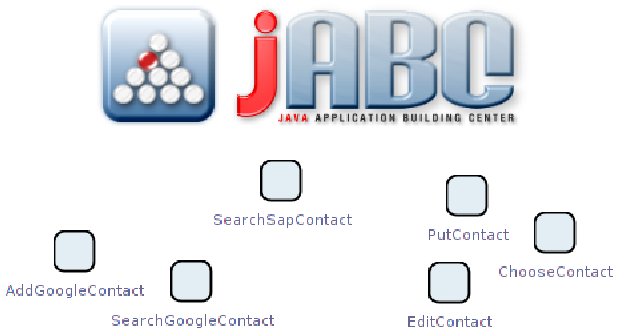
\includegraphics[width=\textheight]{Bilder/titel_sibs.png}
	\end{center}
\end{frame}


\begin{frame}{Vorüberlegungen...}
\begin{itemize}
	\item \textbf{3 Sorten von SIBs:} Google, SAP, GUI
	\pause
	\item \textbf{Google-SIBs:} Kontakt suchen und hinzufügen
	\item \textbf{SAP-SIB:} Kontakt suchen
	\pause
	\item \textbf{GUI-SIBs:}
		\begin{itemize}
			\item Eingabe von Kontakt-Attributen
			\item Auswahl aus einer Liste von Kontakten
		\end{itemize}

\end{itemize}
\end{frame}



\subsection*{SIBs im Detail}
\begin{frame}{Google + SAP: suche Kontakt}
\begin{itemize}
	\item \textbf{Input:} eine Instanz der Klasse \texttt{Contact}
		\begin{itemize}
			\item dient als Filter für die Suche
		\end{itemize}
	\item \textbf{Output:} Liste von \texttt{Contact}-Objekten

	\item \textbf{Branches:}
		\begin{itemize}
			\item \textbf{found:} mindestens ein Kontakt gefunden
			\item \textbf{not found:} keine Ergebnisse
			\item \textbf{error:} es wurde eine \texttt{Exception} geworfen
		\end{itemize}

\end{itemize}
\end{frame}


\begin{frame}{Google: Kontakt hinzufügen}
\begin{itemize}
	\item \textbf{Input:} eine Instanz der Klasse \texttt{Contact}

	\item \textbf{Output:} keiner

	\item \textbf{Branches:}
		\begin{itemize}
			\item \textbf{default:} Kontakt erfolgreich hinzugefügt
			\item \textbf{error:} es wurde eine \texttt{Exception} geworfen
		\end{itemize}

\end{itemize}
\end{frame}


\begin{frame}{GUI: Kontakt-Daten eingeben}
\begin{itemize}
	\item \textbf{Input:} eine Instanz der Klasse \texttt{Contact}
		\begin{itemize}
			\item Formular wird entsprechend befüllt
			\item zudem Parameter für Fenstertitel und Validierung der Eingabe
		\end{itemize}
	\pause
	\item \textbf{Output:} geänderte(!) Instanz der Klasse \texttt{Contact}
		\begin{itemize}
			\item wenn Button "`OK"' geklickt wurde
		\end{itemize}
	\pause
	\item \textbf{Branches:}
		\begin{itemize}
			\item \textbf{ok:} Eingabe bestätigt mit Button "`OK"'
			\item \textbf{cancel:} Eingabe abgebrochen mit Button "`CANCEL"'
			\item \textbf{error:} es wurde eine \texttt{Exception} geworfen, oder \texttt{UNKNOWN}
		\end{itemize}

\end{itemize}
\end{frame}


\begin{frame}{GUI: Kontakt-auswählen}
\begin{itemize}
	\item \textbf{Input:} Liste von \texttt{Contact}-Objekten
		\begin{itemize}
			\item zudem Parameter für Fenstertitel
		\end{itemize}
	\item \textbf{Output:} eine Instanz der Klasse \texttt{Contact}
		\begin{itemize}
			\item wenn Button "`OK"' geklickt wurde
		\end{itemize}

	\item \textbf{Branches:}
		\begin{itemize}
			\item \textbf{ok:} Eingabe bestätigt mit Button "`OK"'
			\item \textbf{cancel:} Eingabe abgebrochen mit Button "`CANCEL"'
			\item \textbf{error:} es wurde eine \texttt{Exception} geworfen, oder \texttt{UNKNOWN}
		\end{itemize}

\end{itemize}
\end{frame}


\subsection*{Probleme während der Entwicklung}
\begin{frame}[fragile]{Besonderheit der GUI-Programmierung}
\begin{itemize}
	\item \textbf{warten auf Eingabe:} wie \texttt{trace()}-Methode anhalten?
		\begin{itemize}
			\item Swing-Frame läuft in einem eigenem Thread!
		\end{itemize}
	\pause
	\item \textbf{Lösung hier:} mittels \texttt{synchronized}-Block in Frame und SIB
\end{itemize}

	\begin{block}{Thread-Synchronisation}
	\javalstset
	\begin{lstlisting}
	public String trace(ExecutionEnvironment env) {
		...
		synchronized (frame) {
			frame.wait();
			...
	\end{lstlisting}
	\end{block}

\begin{itemize}
	\item \textbf{Vorgehen:}
		\begin{itemize}
			\item \texttt{trace()} erstellt den Frame und wartet auf ein \texttt{notify()}
			\item \texttt{notify()} wird vom Action-Listener der Buttons aufgerufen
			\item im Anschluss kann \texttt{trace()} die Eingabe im Frame abfragen
		\end{itemize}
\end{itemize}
\end{frame}



\begin{frame}[fragile]{Eigener Code im jABC}
\begin{itemize}
	\item \textbf{Unterschiede in der Laufzeitumgebung:} 
	\begin{itemize}
			\item Code läuft ausserhalb von jABC...
			\item ABER: Ausführung des Graphen wirft \texttt{Exception}?
	\end{itemize}
	\pause
	\item \textbf{Lösung hier:} mittels "`\underline{bad} Practice"'
\end{itemize}

\begin{block}{Änderung von Systemeigenschaften}
\javalstset
\begin{lstlisting}
...
System.setProperty("javax.xml.parsers.SAXParser", ...);
System.setProperty("...parsers.SAXParserFactory", ...);
System.setProperty("oracle.xml.parser.v2.SAXParser...);
...
\end{lstlisting}
\end{block}

\begin{itemize}
	\item \textbf{Effekt:}
		\begin{itemize}
			\item konfiguriert aktiv laufende JVM
			\item auch nach Ausführung des Modells weiterhin wirksam
			\item sollte in realem Szenario vermieden werden!
		\end{itemize}
\end{itemize}
\end{frame}


\section{jABC-Modell}

\subsection*{}
\begin{frame}{Der Modell-Graph im jABC}
\begin{center}
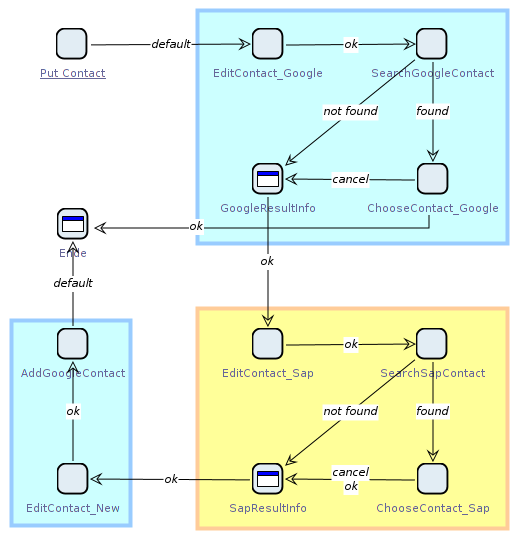
\includegraphics[height=0.8\textheight]{Bilder/jabc_Model.png} 
\end{center}
\end{frame}



